\documentclass[table,aspectratio=169]{beamer}

\usefonttheme{professionalfonts}
\usefonttheme[onlymath]{serif}

\mode<presentation>
{
  \usetheme{CambridgeUS}
  \setbeamercolor{item projected}{bg=darkred}
  \setbeamertemplate{enumerate items}[default]
  \setbeamertemplate{navigation symbols}{}
  \setbeamertemplate{itemize item}{-}
  \setbeamertemplate{itemize subitem}[triangle]
  \setbeamercovered{transparent}
  \setbeamercolor{block title}{fg=darkred}
  \setbeamercolor{local structure}{parent=alerted text}
}
\addtobeamertemplate{block begin}{\setbeamercolor{local structure}{parent=structure}}{}

\usepackage[english]{babel}
\usepackage{amssymb}
\usepackage{mathcmd}
\usepackage{nicefrac}
\usepackage{booktabs}
\usepackage{graphicx}
\usepackage{siunitx}
\usepackage{bbm}
\usepackage{url}
\usepackage{acronym}
\graphicspath{{./}{./../talk_plots/}{./../../plots/}}

%\usepackage{courier}
%\usepackage{times}
% The non-standard packages arev and bera define fonts which look nicely for
% projection, you might want to try them instead of Times/Helvetica/Courier.
% Use the

\acrodef{ICAO}{International Civil Aviation Organization}

%%%%%%%%%%%%%%%%%%%%%%%%%%%%%%%%%%%%%%%%%%%%%%%%%%%%%%%%%%%%%%%%%%%%%%%%
\usepackage{pxfonts} % Or palatino or mathpazo
\usepackage{eulervm}
\linespread{1.05}
%%%%%%%%%%%%%%%%%%%%%%%%%%%%%%%%%%%%%%%%%%%%%%%%%%%%%%%%%%%%%%%%%%%%%%%%
\usepackage[T1]{fontenc}
% Or whatever. Note that the encoding and the font should match. If T1
% does not look nice, try deleting the line with the fontenc.
\usepackage{hyperref}

\newcommand{\prob}[1]{\ensuremath{\mathbb{P}\left(  #1 \right)}}
\newcommand{\mean}[1]{\ensuremath{\mathbb{E}\left(  #1 \right)}}
\newcommand\independent{\protect\mathpalette{\protect\independenT}{\perp}}
\newcommand{\menquote}[1]{\ensuremath{\text{\textquotedbl} #1 \text{\textquotedbl}}}
\def\independenT#1#2{\mathrel{\rlap{\(#1#2\)}\mkern2mu{#1#2}}}

\definecolor{eham}{rgb}{1.0, 0.714, 0.467}
\definecolor{egll}{rgb}{0.427, 0.714, 1.0}
\definecolor{egss}{rgb}{0.859, 0.82, 0.0}
\definecolor{lgav}{rgb}{0.0, 0.427, 0.859}
\definecolor{lemd}{rgb}{0.573, 0.0, 0.0}
\definecolor{egkk}{rgb}{0.0, 0.286, 0.286}
\definecolor{lirf}{rgb}{0.141, 1.0, 0.141}
\definecolor{eddf}{rgb}{0.286, 0.0, 0.573}
\definecolor{eggw}{rgb}{0.714, 0.859, 1.0}
\definecolor{lfpg}{rgb}{0.573, 0.286, 0.0}

\newcommand{\airp}[1]{\textcolor{#1}{\textsc{#1}}}


%\setbeamerfont{alerted text}{series=\scshape}

\title[Data-driven modelling for inbound air traffic]{Data-driven modelling and validation of the inbound flow\\
at some major European airports}
% \subtitle{}

\author[Carlo Lancia]{Carlo Lancia \inst{1} \and Guglielmo Lulli \inst{2}}

\institute[Leiden Univ.]{\inst{1} Mathematical Institute Leiden University,\\
                         \inst{2} Lancaster University Management School}

\date[ECSO 2017]{ECSO 2017, August 22, 2017}
% - Either use conference name or its abbreviation.
% - Not really informative to the audience, more for people (including
%   yourself) who are reading the slides online

% \usepackage{hyperref}
% \subject{Cutoff phenomenon for finite Markov chains}
% This is only inserted into the PDF information catalog. Can be left
% out.

% \AtBeginSection[]
% {
%   \begin{frame}<beamer>
%     \frametitle{Outline}
%     \tableofcontents[currentsection,hideothersubsections]
%   \end{frame}
% }
% Use this if you do want the table of contents to pop up at
% the beginning of each subsection.

% \pgfdeclareimage[height=2em,interpolate=true]{ntnulogotext}{foo}
% If you want to include a different logo on the title page
% only (e.g. a combined logo of different institutions), you
% can use this command.

% -------------------------------------
% \includeonlyframes{current}
% -------------------------------------

\begin{document}

\maketitle
% You can use \maketitle to create the titlepage,
% or \compressedtitle to create a more compact titlepage
% with the look of the other pages in compress style

% \begin{frame}
%   \titlepage
% \end{frame}
% Or you can call the titlepage command in a frame environment

% \begin{frame}<beamer>[label=current]
%   \frametitle{Outline}
%   \tableofcontents[hideallsubsections]
% \end{frame}

\begin{frame}[t]\frametitle{Summary}
    \begin{alertblock}{Problem}
        Estimating the daily demand at major European airports
    \end{alertblock}

    \begin{alertblock}{Data and Methods}
        \begin{itemize}
            \item Entrance time in a cylinder of radius 40 NM around airport
            \item Data-driven definition of Poisson process and Pre-scheduled Random Arrivals
            \item Comparison of the two processes
        \end{itemize}
    \end{alertblock}

    \begin{alertblock}{Conclusions}
        PSRA should be preferred whenever mathematical tractability is not an issue
    \end{alertblock}
\end{frame}

\begin{frame}[t]\frametitle{Modelling the length of inbound queue at Heathrow (\airp{egll})}
    \begin{center}
        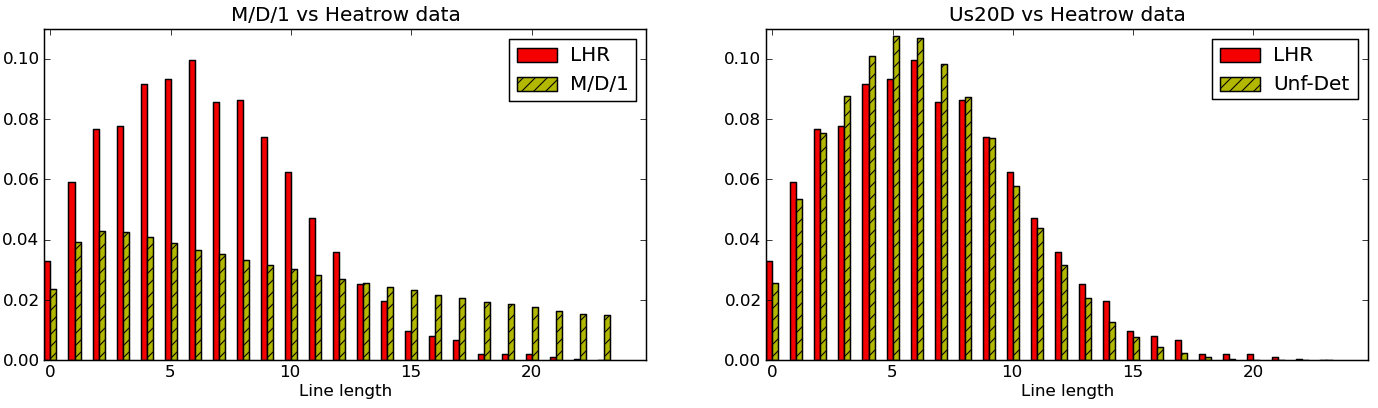
\includegraphics[width=.8\textwidth]{cills}

        {\tiny From Caccavale, Iovanella, \textbf{Lancia}, \textbf{Lulli}, Scoppola (2014)
        A model of inbound air traffic: The application to Heathrow airport.\\
        \emph{Journal of Air Transport Management}, 34, 116--122}
    \end{center}
\end{frame}

\begin{frame}[t]\frametitle{Pre-scheduled random arrivals}
    \centering
    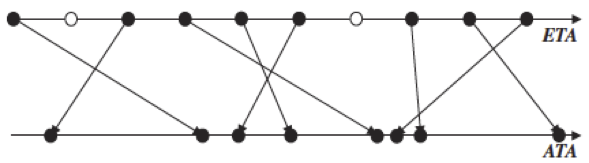
\includegraphics[width=.65\textwidth]{psra}

    {\tiny From Caccavale et al. (2014) \emph{J Air Transp Manag}, 34, 116--122}

    \vfill

    \begin{alertblock}{Idea}
        Fixed, deterministic schedule perturbed by IID random variables
        \[ t_i = \frac{i}{\mu} + \xi_i \]
        Optional thinning process (hollow dots)
    \end{alertblock}
\end{frame}

\begin{frame}[t]\frametitle{Poisson and PSRA model}
    \centering
    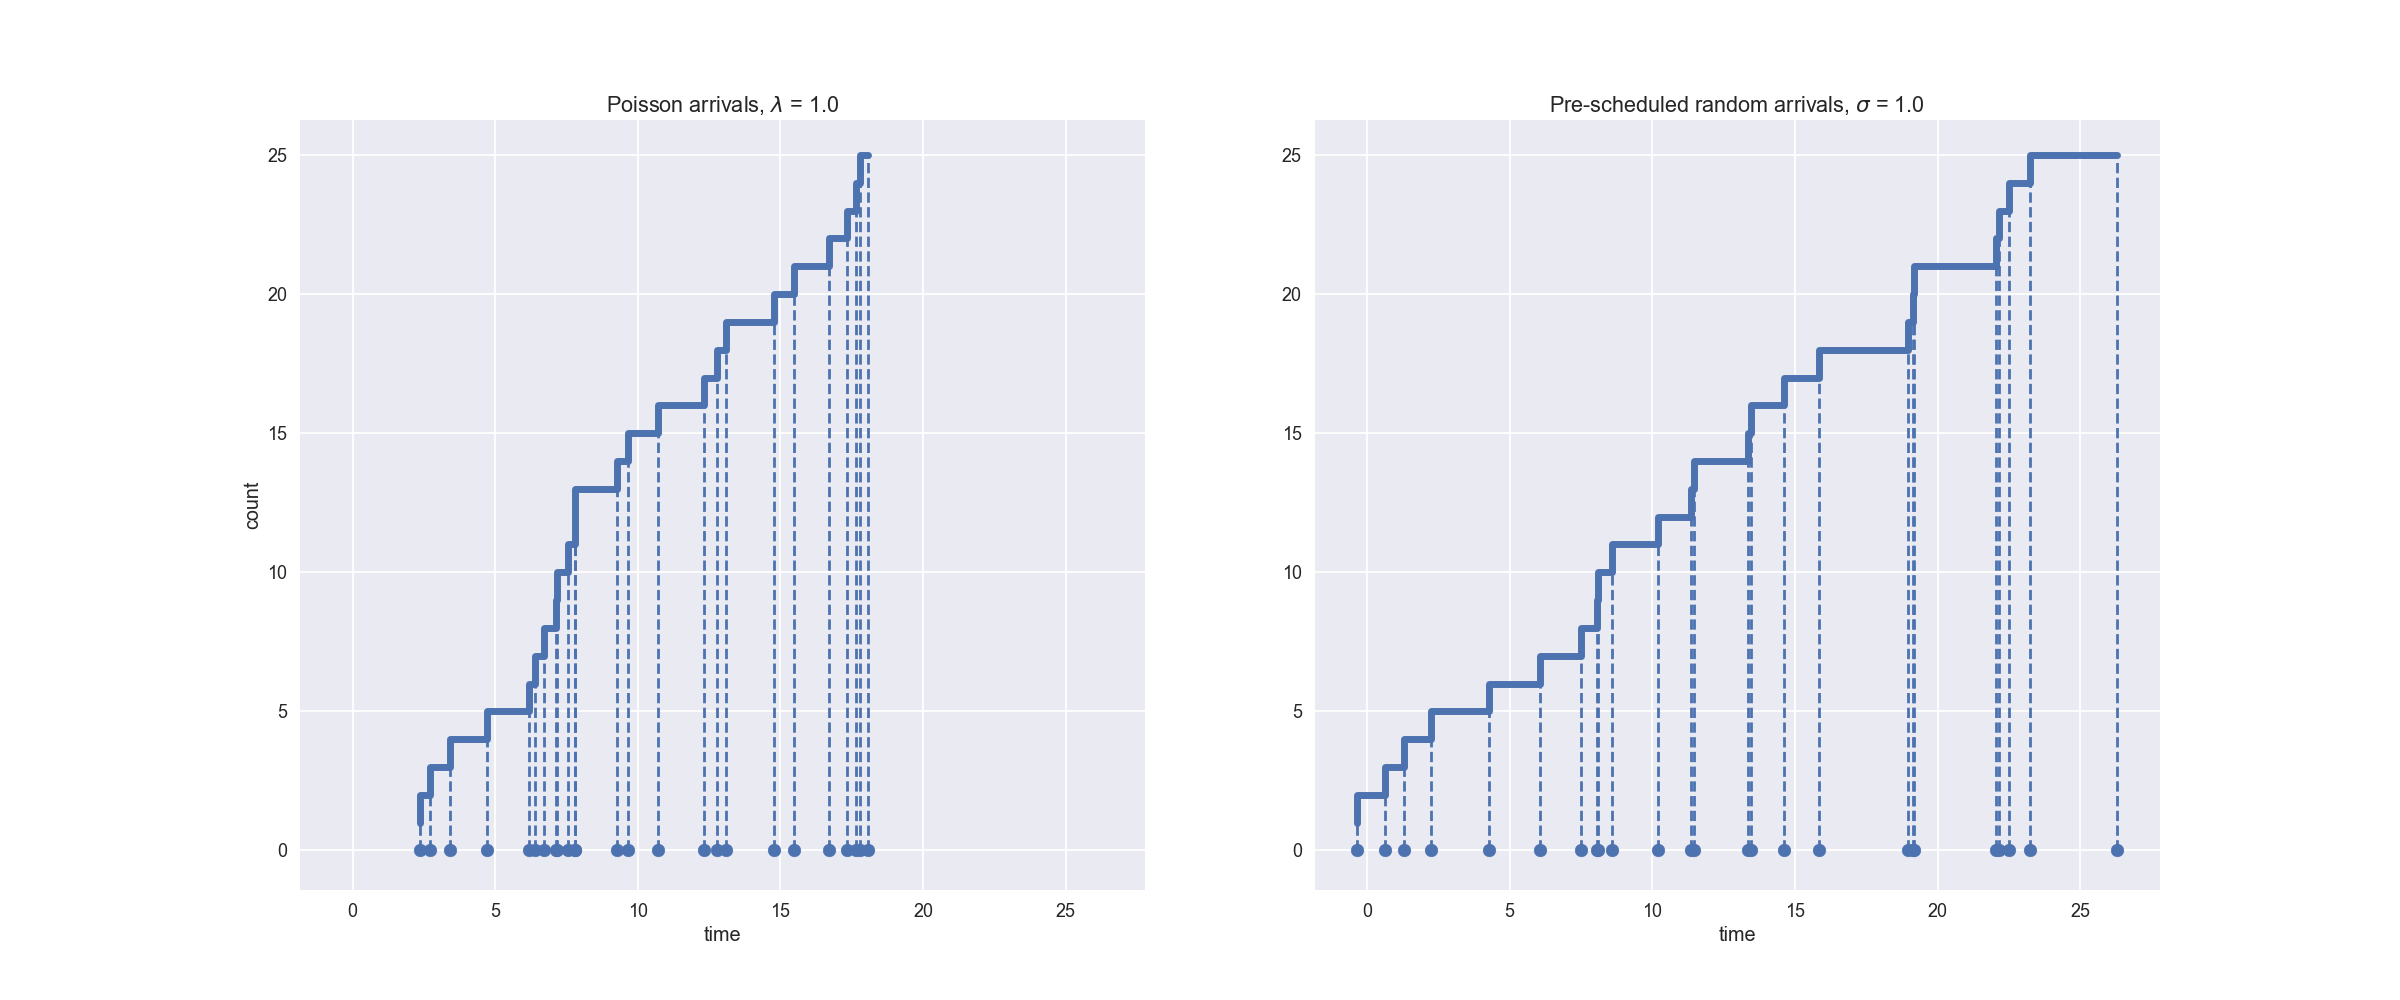
\includegraphics[width=.9\textwidth]{pois_psra}
    \vfill
    \alert{$\cdot$/D/1 queue model:} single server, deterministic service time
\end{frame}

\begin{frame}[t]\frametitle{Modelling the length of inbound queue at Heathrow (\airp{egll})}
    \begin{columns}
        \column{.6\textwidth}
        \begin{center}
            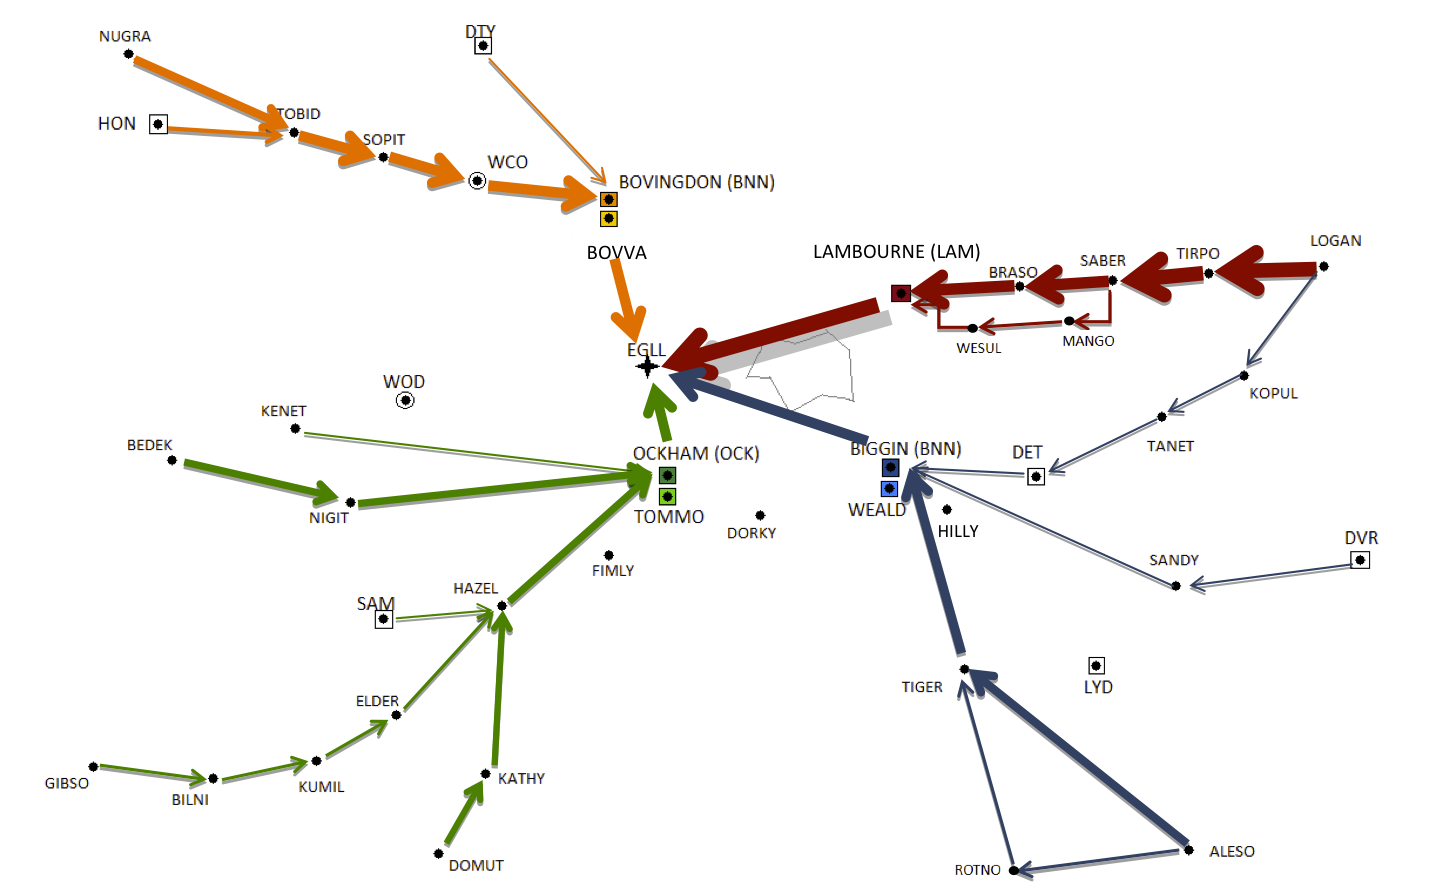
\includegraphics[width=.85\textwidth]{cills2}

            {\tiny From Caccavaleet al. (2014) \emph{J Air Transp Manag}, 34, 116--122}
        \end{center}
        \column{.4\textwidth}
        \begin{itemize}
            \item Indirect comparison with Poisson, i.e.\ through a queueing model
            \item Analysis overlooks action of TC on inbound stream
            \item \emph{This leads to overestimating PSRA parameter $\sigma$}
            \item Deterministic schedule of PSRA is equally spaced in time (this is ok for \airp{egll}, though)
        \end{itemize}
    \end{columns}
\end{frame}

\begin{frame}[t]\frametitle{Dataset overview}
    \centering
    \begin{tabular}{lcr}
\toprule
{} & \acs{ICAO} code &  sample size \\
airport name                            &                 &              \\
\midrule
Frankfurt am Main International Airport &     \airp{eddf} &        58167 \\
London Gatwick Airport                  &     \airp{egkk} &        39746 \\
London Heathrow Airport                 &     \airp{egll} &        56716 \\
Amsterdam Airport Schiphol              &     \airp{eham} &        63279 \\
Madrid Barajas International Airport    &     \airp{lemd} &        48162 \\
Charles de Gaulle International Airport &     \airp{lfpg} &        60122 \\
Athens International Airport            &     \airp{lgav} &        29503 \\
Rome Fiumicino International Airport    &     \airp{lirf} &        43333 \\
\bottomrule
\end{tabular}


    \vfill

    \alert{Study period} goes from June 15 to September 15, 2016

    \alert{We model the demand} using first time within 40 NM from airport
\end{frame}

\begin{frame}[t]\frametitle{Average daily demand}
    \centering
    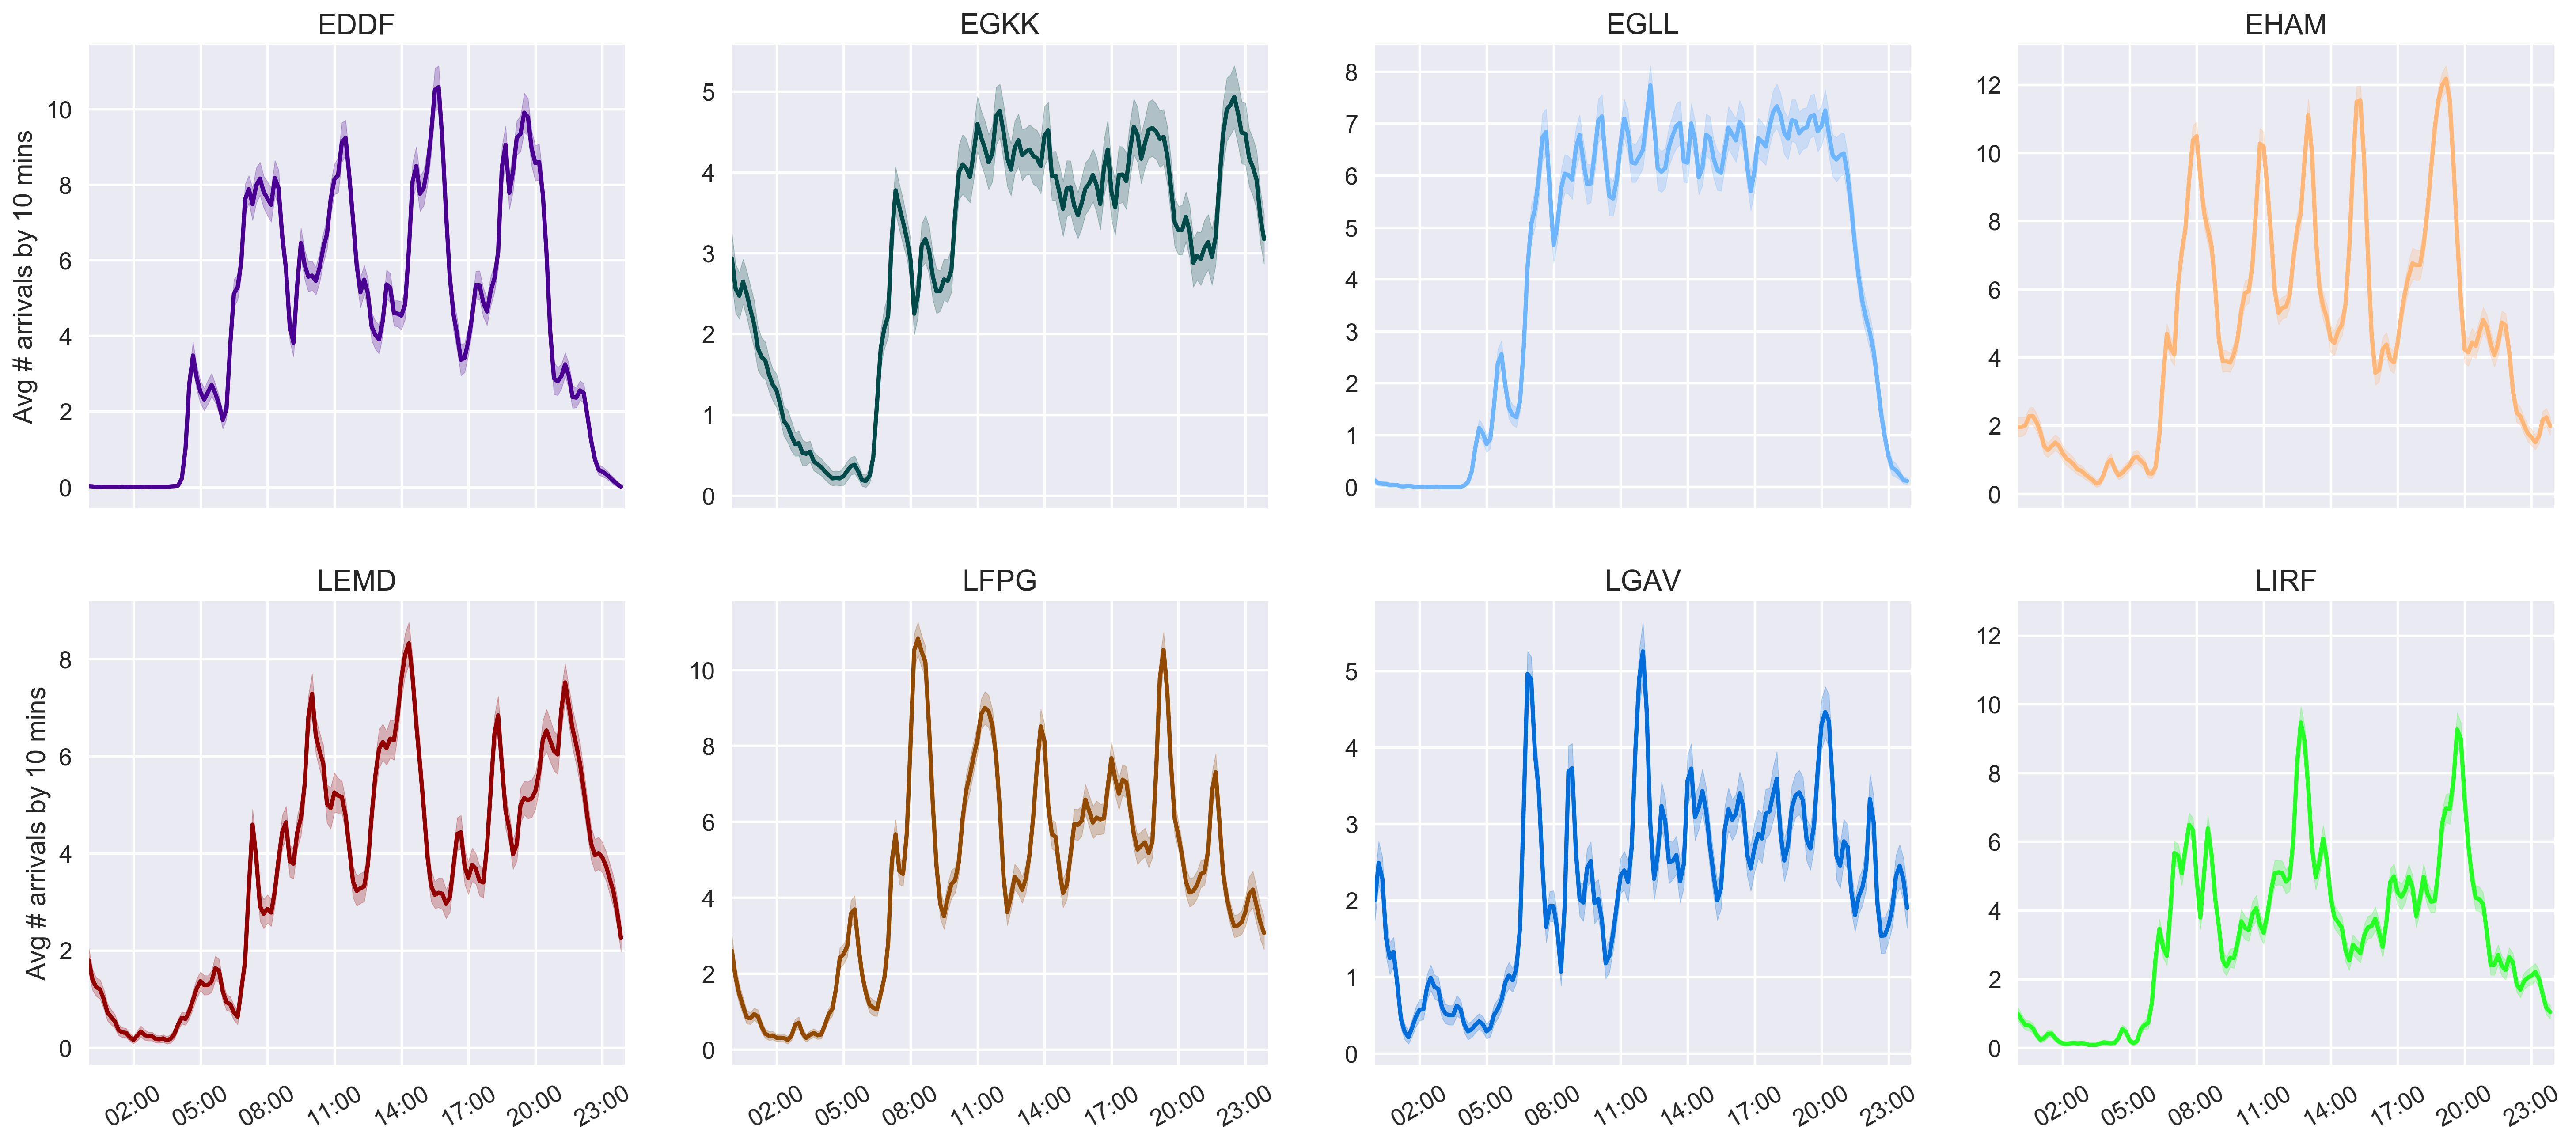
\includegraphics[width=.9\textwidth]{AvgArrivals}
\end{frame}

\begin{frame}[t]\frametitle{Daily periodicity}
    \centering
    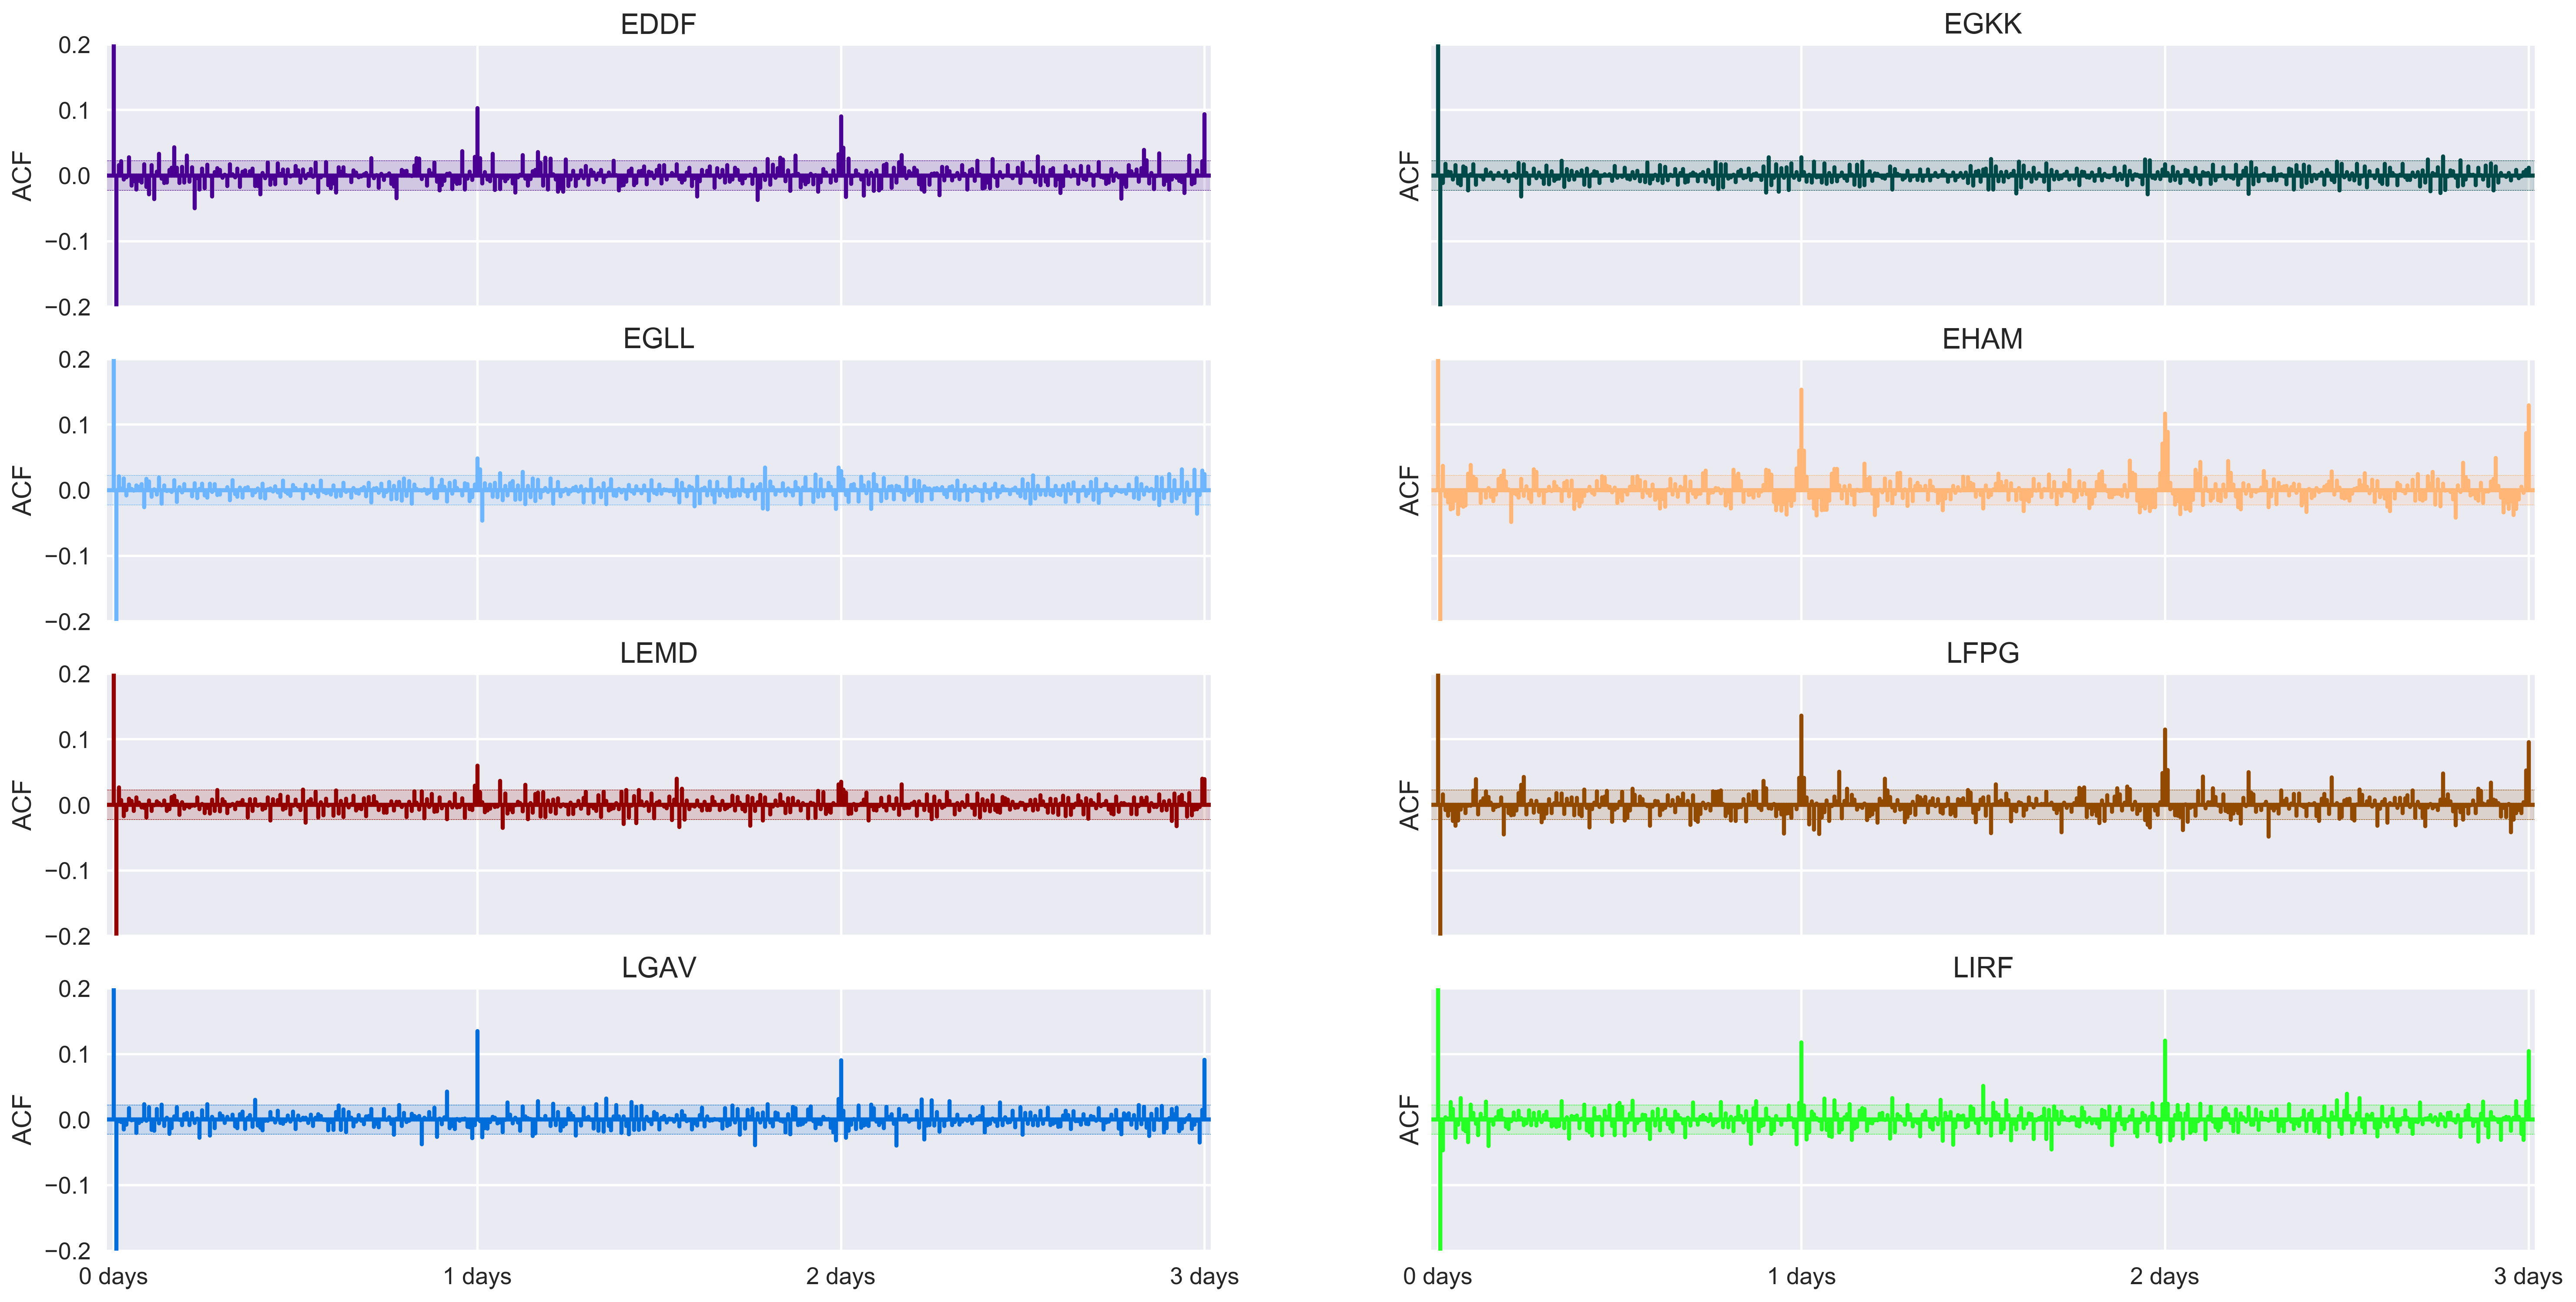
\includegraphics[width=.8\textwidth]{Autocorr}
\end{frame}

\begin{frame}[t]\frametitle{Data-driven Poisson process}
    \begin{enumerate}
        \item Aggregate arrivals TS, e.g.\ by intervals of 10 minutes
        \item Run a \alert{changepoint-detection} algorithm, e.g.\ PELT, under the null hypothesis of Poissonian arrivals to obtain
        \begin{itemize}
            \item changepoint time $\hat{t}_k$
            \item $\hat{\lambda}_k$, estimated intensity in $[\hat{t}_k, \hat{t}_{k+1})$
        \end{itemize}
        \item \alert{Cluster} couples $\{(\hat{t}_k, \hat{\lambda}_k)\}_k$, e.g.\ via DBSCAN
        \item Compute the \alert{centroid} $(\bar{t}_i, \bar{\lambda}_i)$ of each cluster
        \item Define a \alert{step-wise, periodic intensity function} that takes on $\bar{\lambda}_i$ for $t \,\in\, [\bar{t}_i, \bar{t}_{i+1})$
    \end{enumerate}
\end{frame}

\begin{frame}[t]\frametitle{Changepoint detection via PELT}
    \begin{columns}
        \column{.5\textwidth}
        \begin{itemize}
            \item PELT is an algorithm for multiple changepoint detection in a time series
            \item It can detect changes in mean, variance, or both
            \item Software available via R package \texttt{changepoint}
            \item We work under the null of Poisson arrivals
        \end{itemize}

        \column{.5\textwidth}
        \centering
        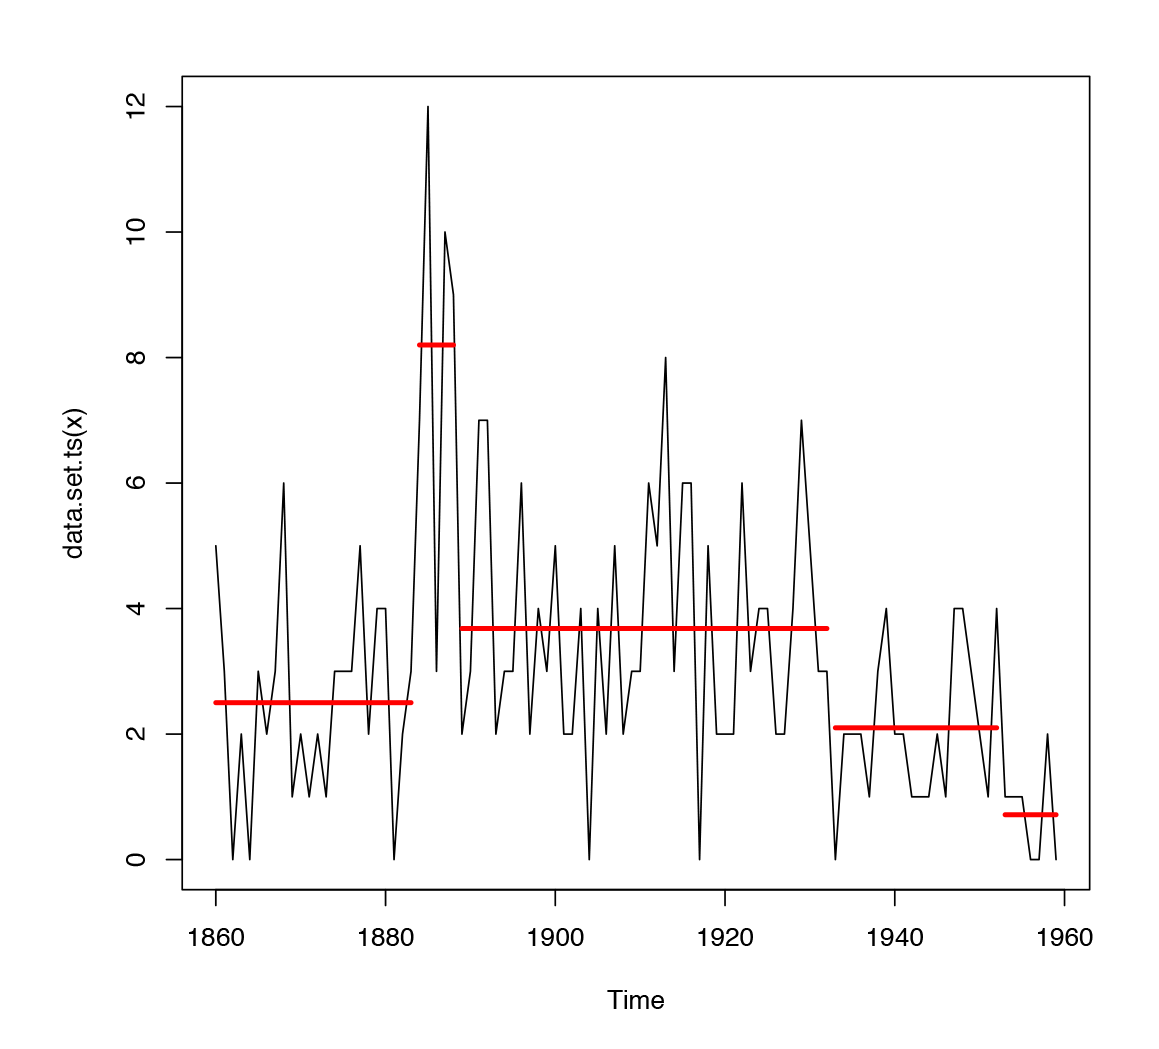
\includegraphics[width=.85\textwidth]{pelt}

        {\tiny Killick, Eckley (2014) \emph{J Stat Soft} 58(3)}
    \end{columns}
\end{frame}

\begin{frame}[t]\frametitle{Clustering via DBSCAN}
    \begin{columns}
        \column{.5\textwidth}
        \begin{itemize}
            \item Density-based spatial clustering of applications with noise (DBSCAN)
            \item Two hyperparameters, $\varepsilon$ and $n_{\mathrm{pts}}$
            \item Core points (red) have at least $n_{\mathrm{pts}}$ other points within distance $\varepsilon$
            \item Non-core (yellow) lie within $\varepsilon$ from a core point
            \item The remainders are outliers (blue)
        \end{itemize}

        \column{.5\textwidth}
        \centering
        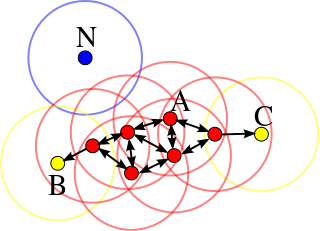
\includegraphics[width=.85\textwidth]{dbscan}

        {\tiny Source: Wikimedia Commons}
    \end{columns}
\end{frame}

\begin{frame}[t]\frametitle{Implementation of data-driven Poisson process}
    \centering
    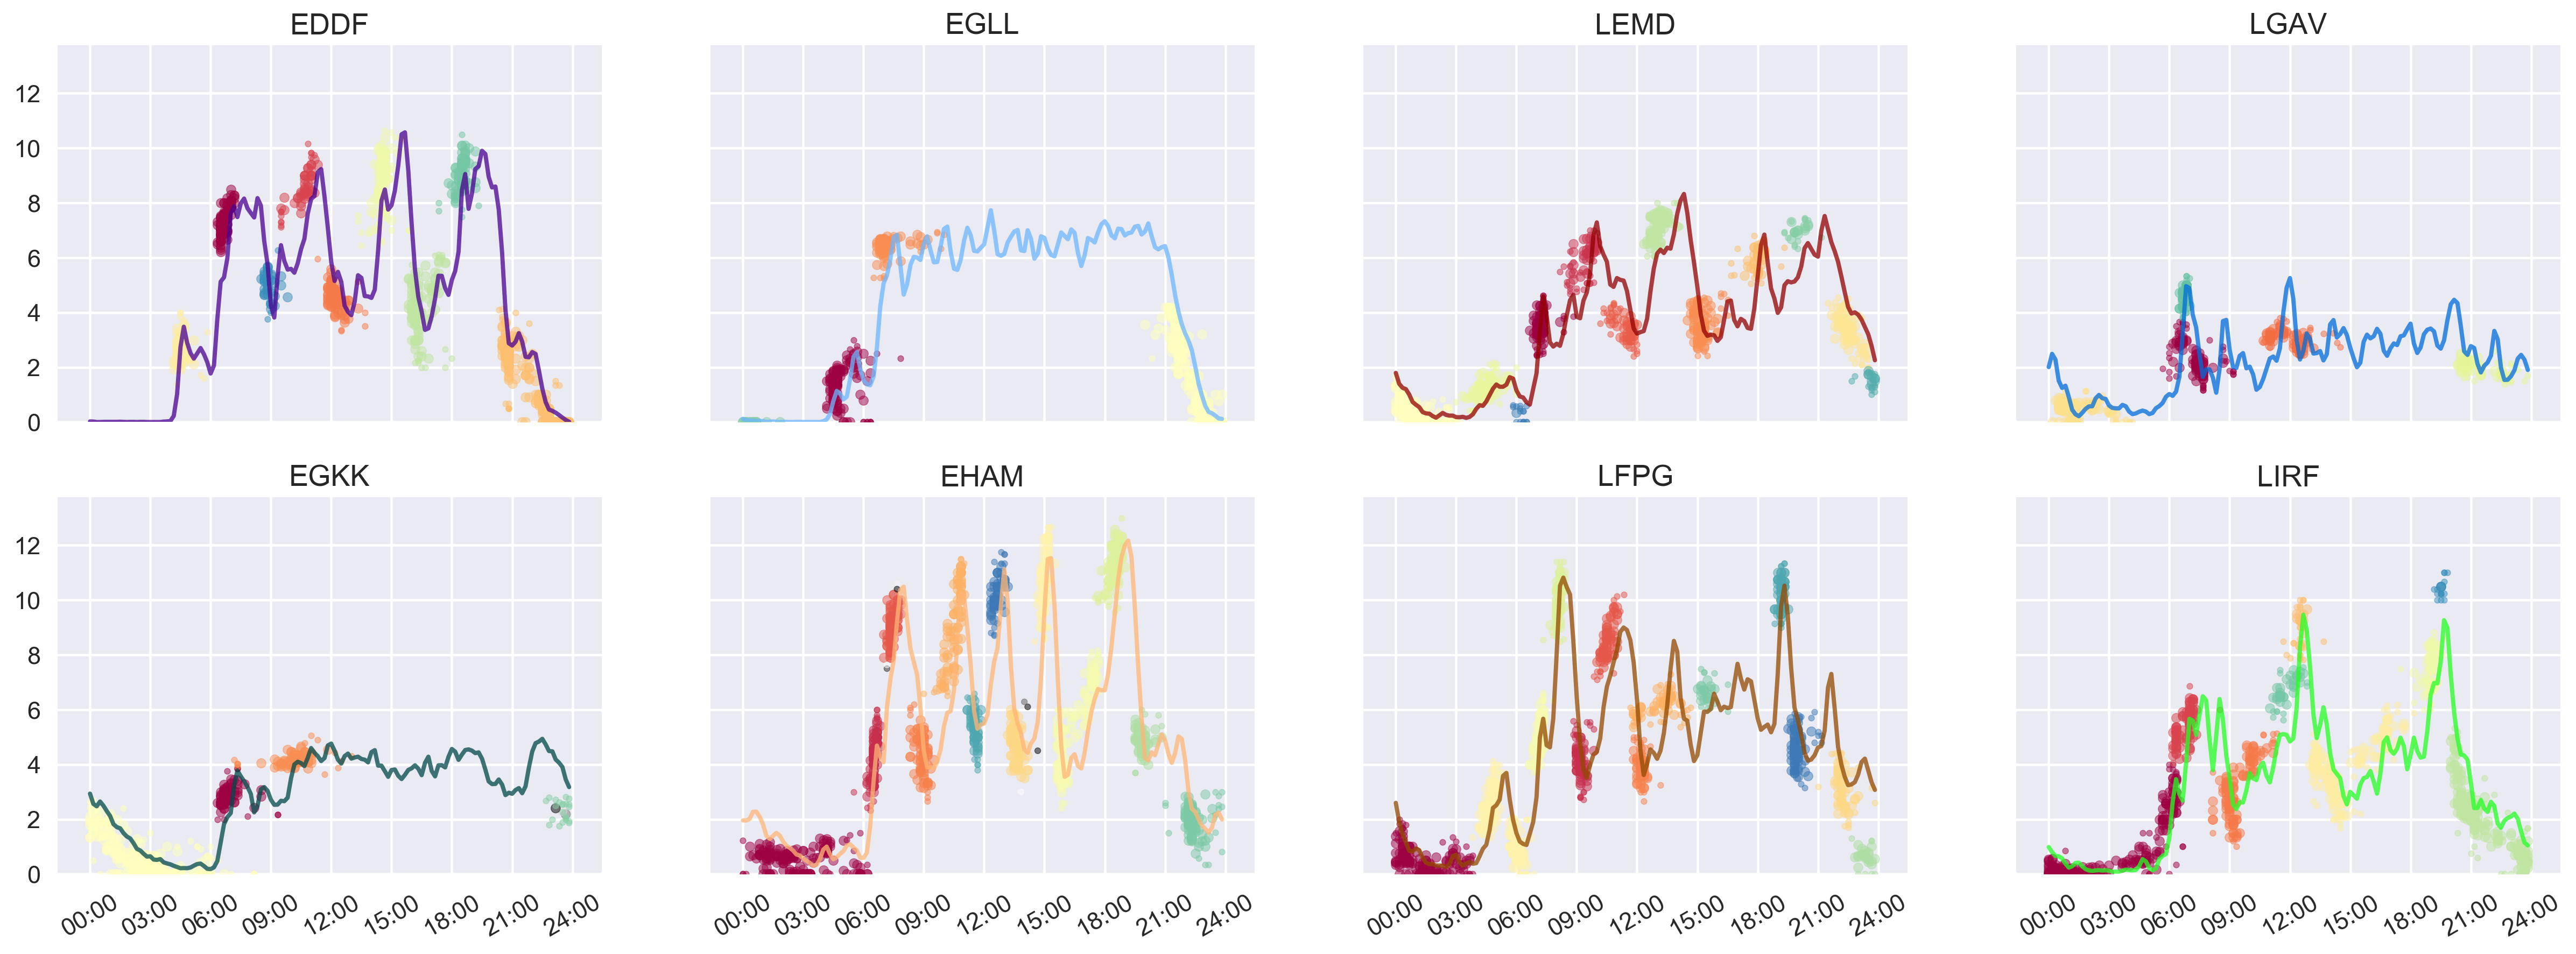
\includegraphics[width=\textwidth]{DDPoisson}
\end{frame}

\begin{frame}[t]\frametitle{Data-driven PSRA}
    \begin{enumerate}
        \item Let $t^{\mathrm{M3}}_i$ the \alert{\emph{actual} arrival} time at 40 NM
        \item Let $t^{\mathrm{M1}}_i$ the \alert{\emph{anticipated} arrival} time at 40 NM (from the last flight plan agreed with Eurocontrol)
        \item Compute the \emph{delays} $\delta_i = t^{\mathrm{M1}_i} - t^{\mathrm{M1}_i}$
        \item Define
        \[t_i = t^{\mathrm{M1}}_i + \xi_i\]
        where $\{\xi_i\}_i$ are IID rvs drawn from the empirical distribution of the delays $\{\delta_i\}_i$
    \end{enumerate}
\end{frame}

\begin{frame}[t]\frametitle{Data-driven Poisson vs PSRA}
    \centering
    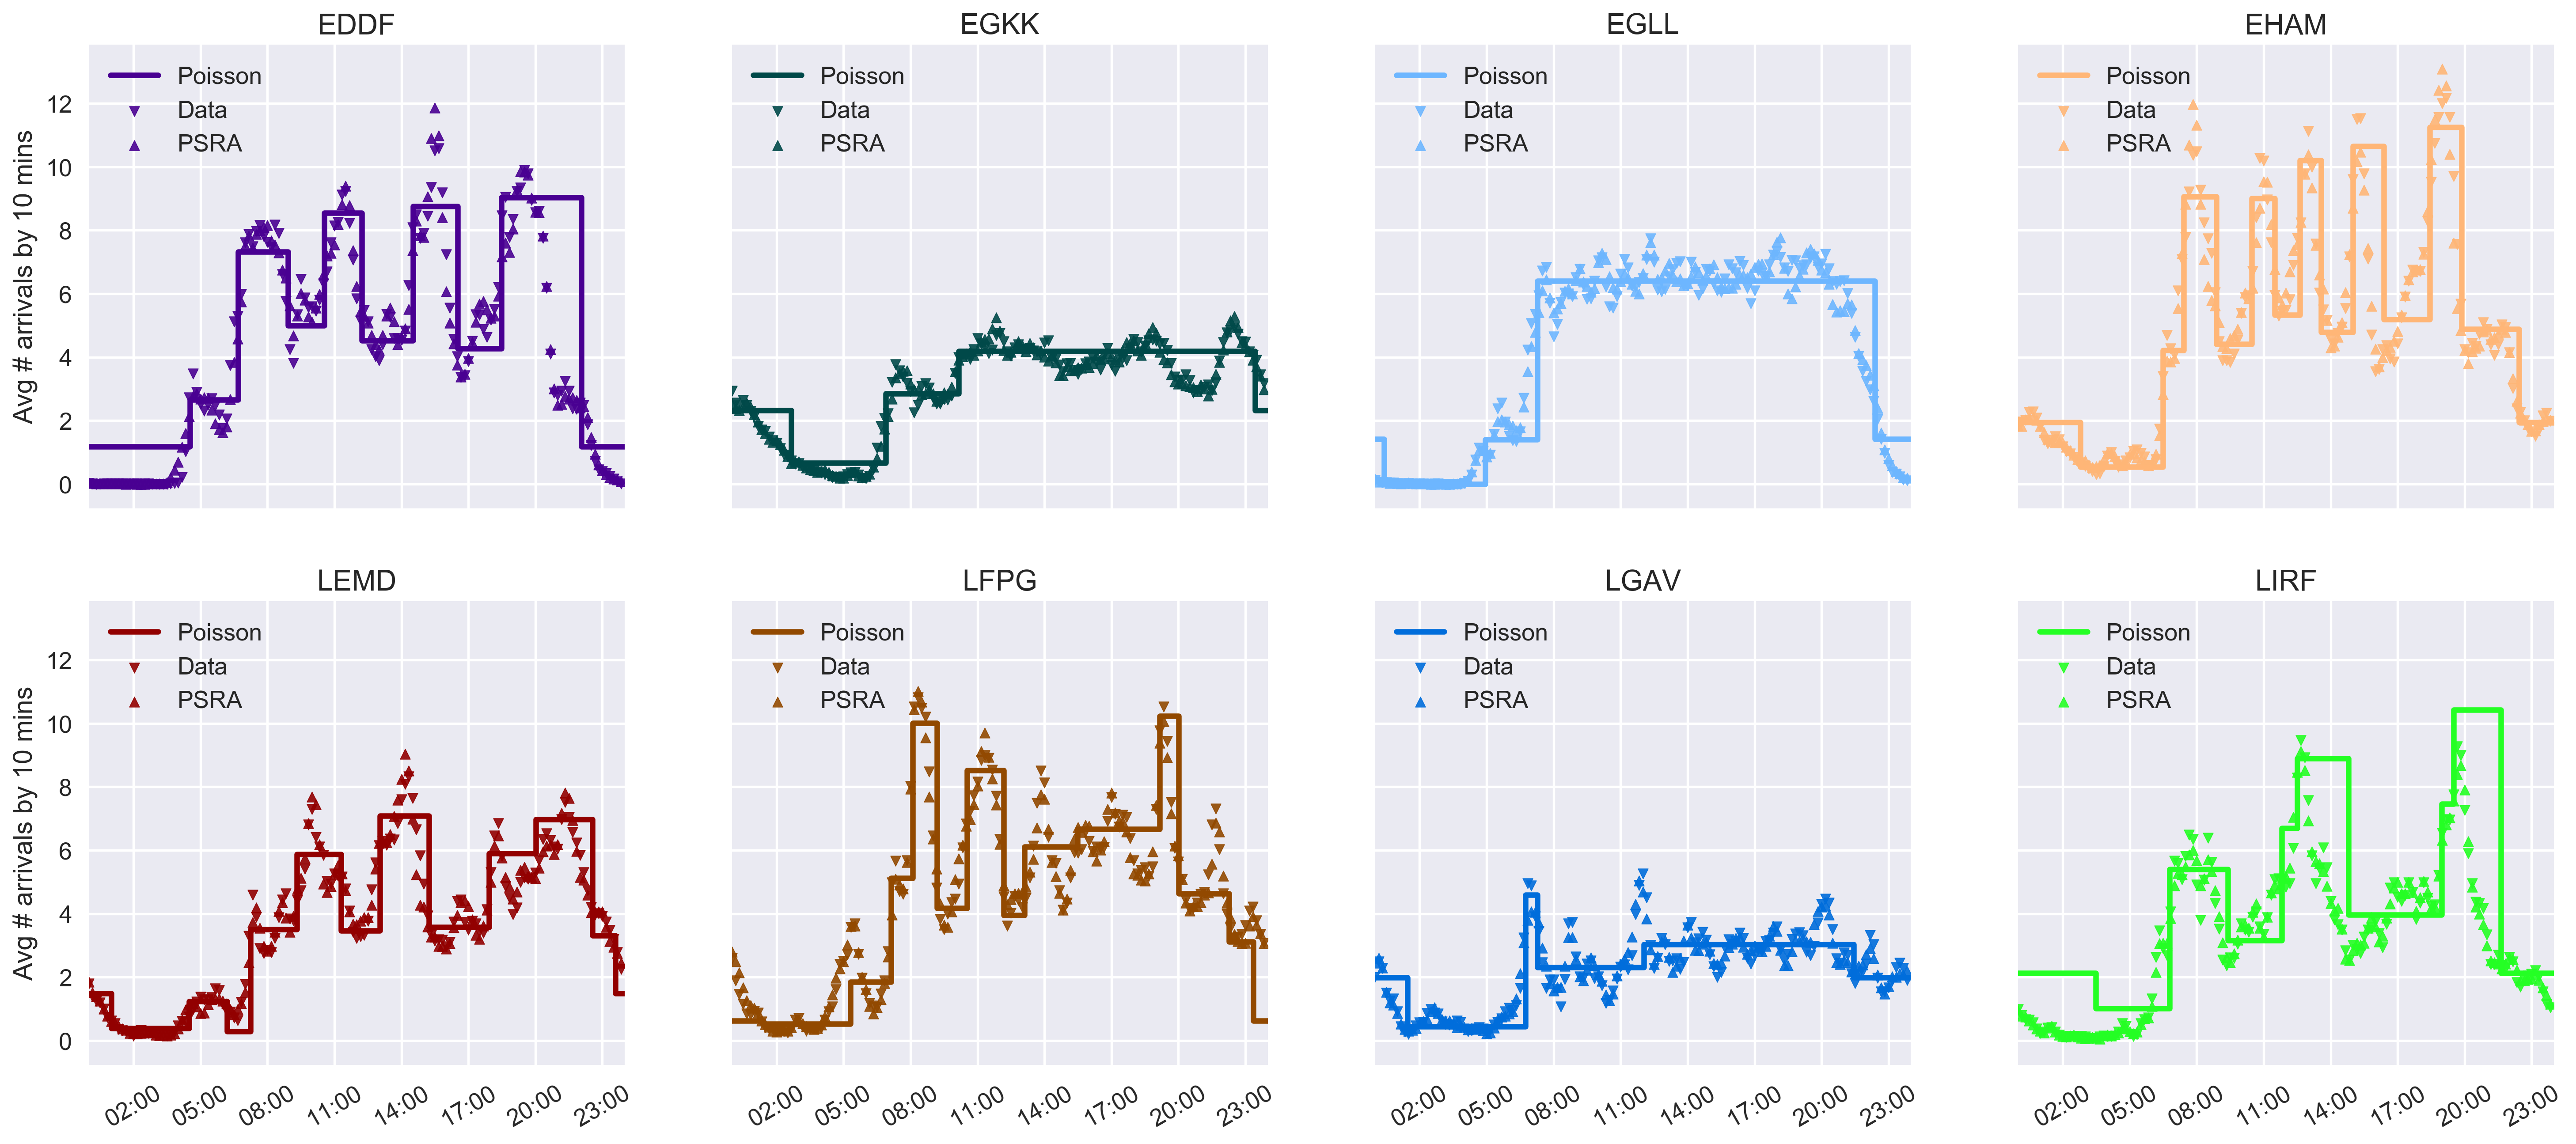
\includegraphics[width=.9\textwidth]{mean_simul_arrivals}
\end{frame}

\begin{frame}[t]\frametitle{Data-driven Poisson vs PSRA}
    \begin{itemize}
        \item PSRA outperform Poisson arrivals in reproducing the average daily demand
        \item Average demand reproduced with Poisson model by \alert{forcing} intensity to vary over a finer time scale
        \begin{itemize}
            \item \alert{CAVEAT} number of parameters requires increases in a sensible manner
        \end{itemize}
        \item PSRA is non-parametric
        \item A semi-parametric model is possible by defining $\xi_i = \xi_i(Z)$
        \item PSRA inherits \alert{arrivals correlation-structure} from the M1 schedule
        \item In contrast, Poissonian arrivals have \alert{independent increments} by definition
    \end{itemize}
\end{frame}

\begin{frame}[t]\frametitle{Arrivals correlation}
    \centering
    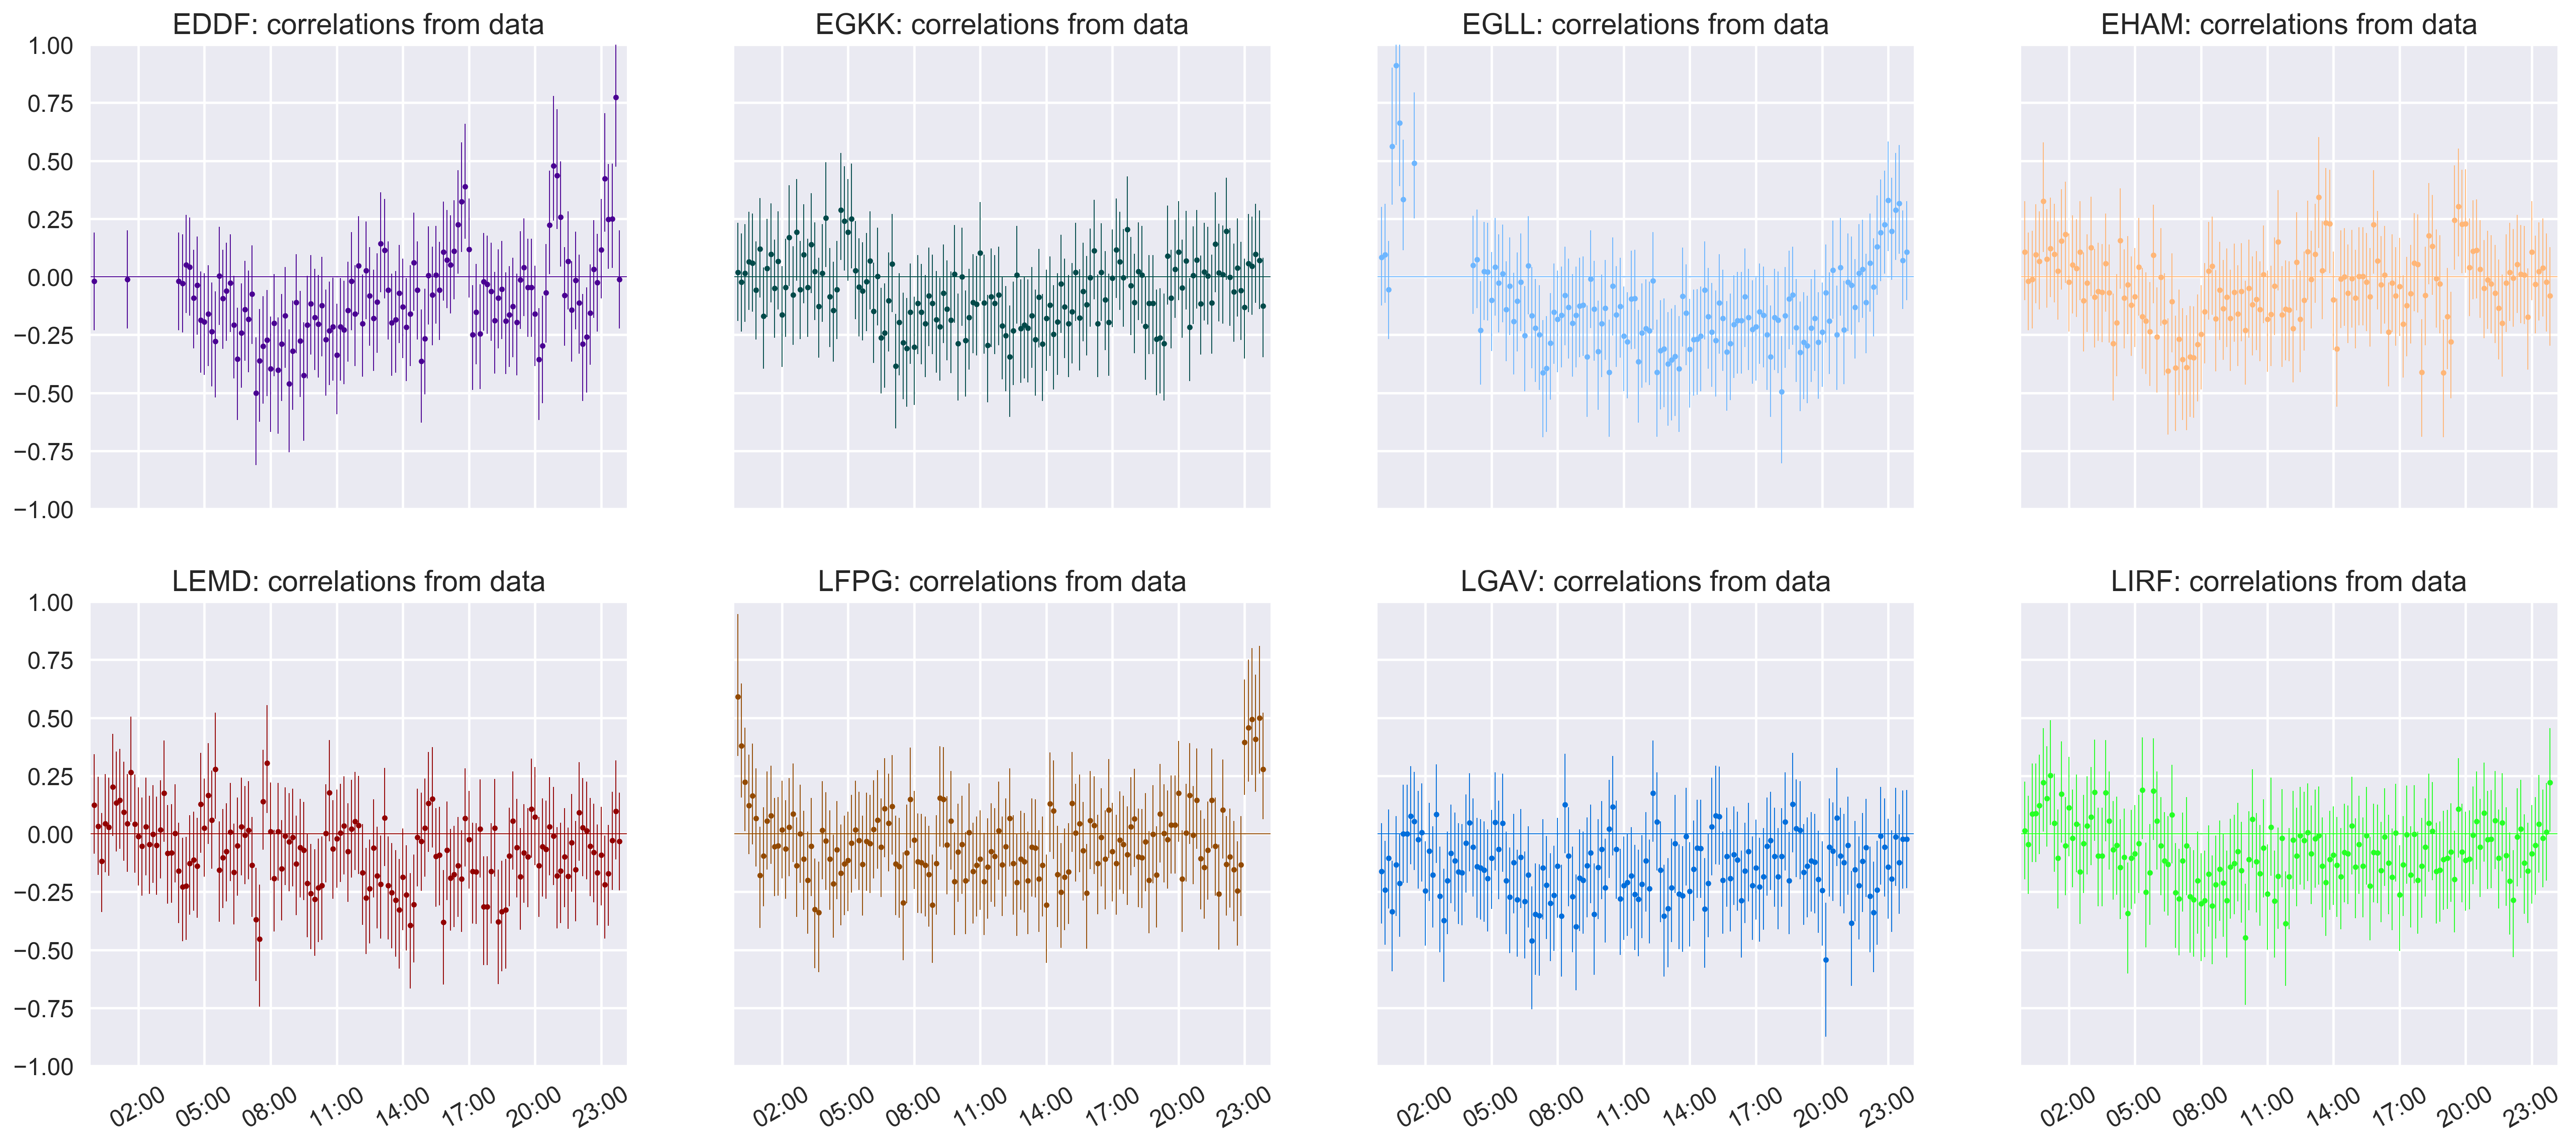
\includegraphics[width=.9\textwidth]{correlations_true}
\end{frame}

\begin{frame}[t]\frametitle{Correlations from simulation of PSRA}
    \centering
    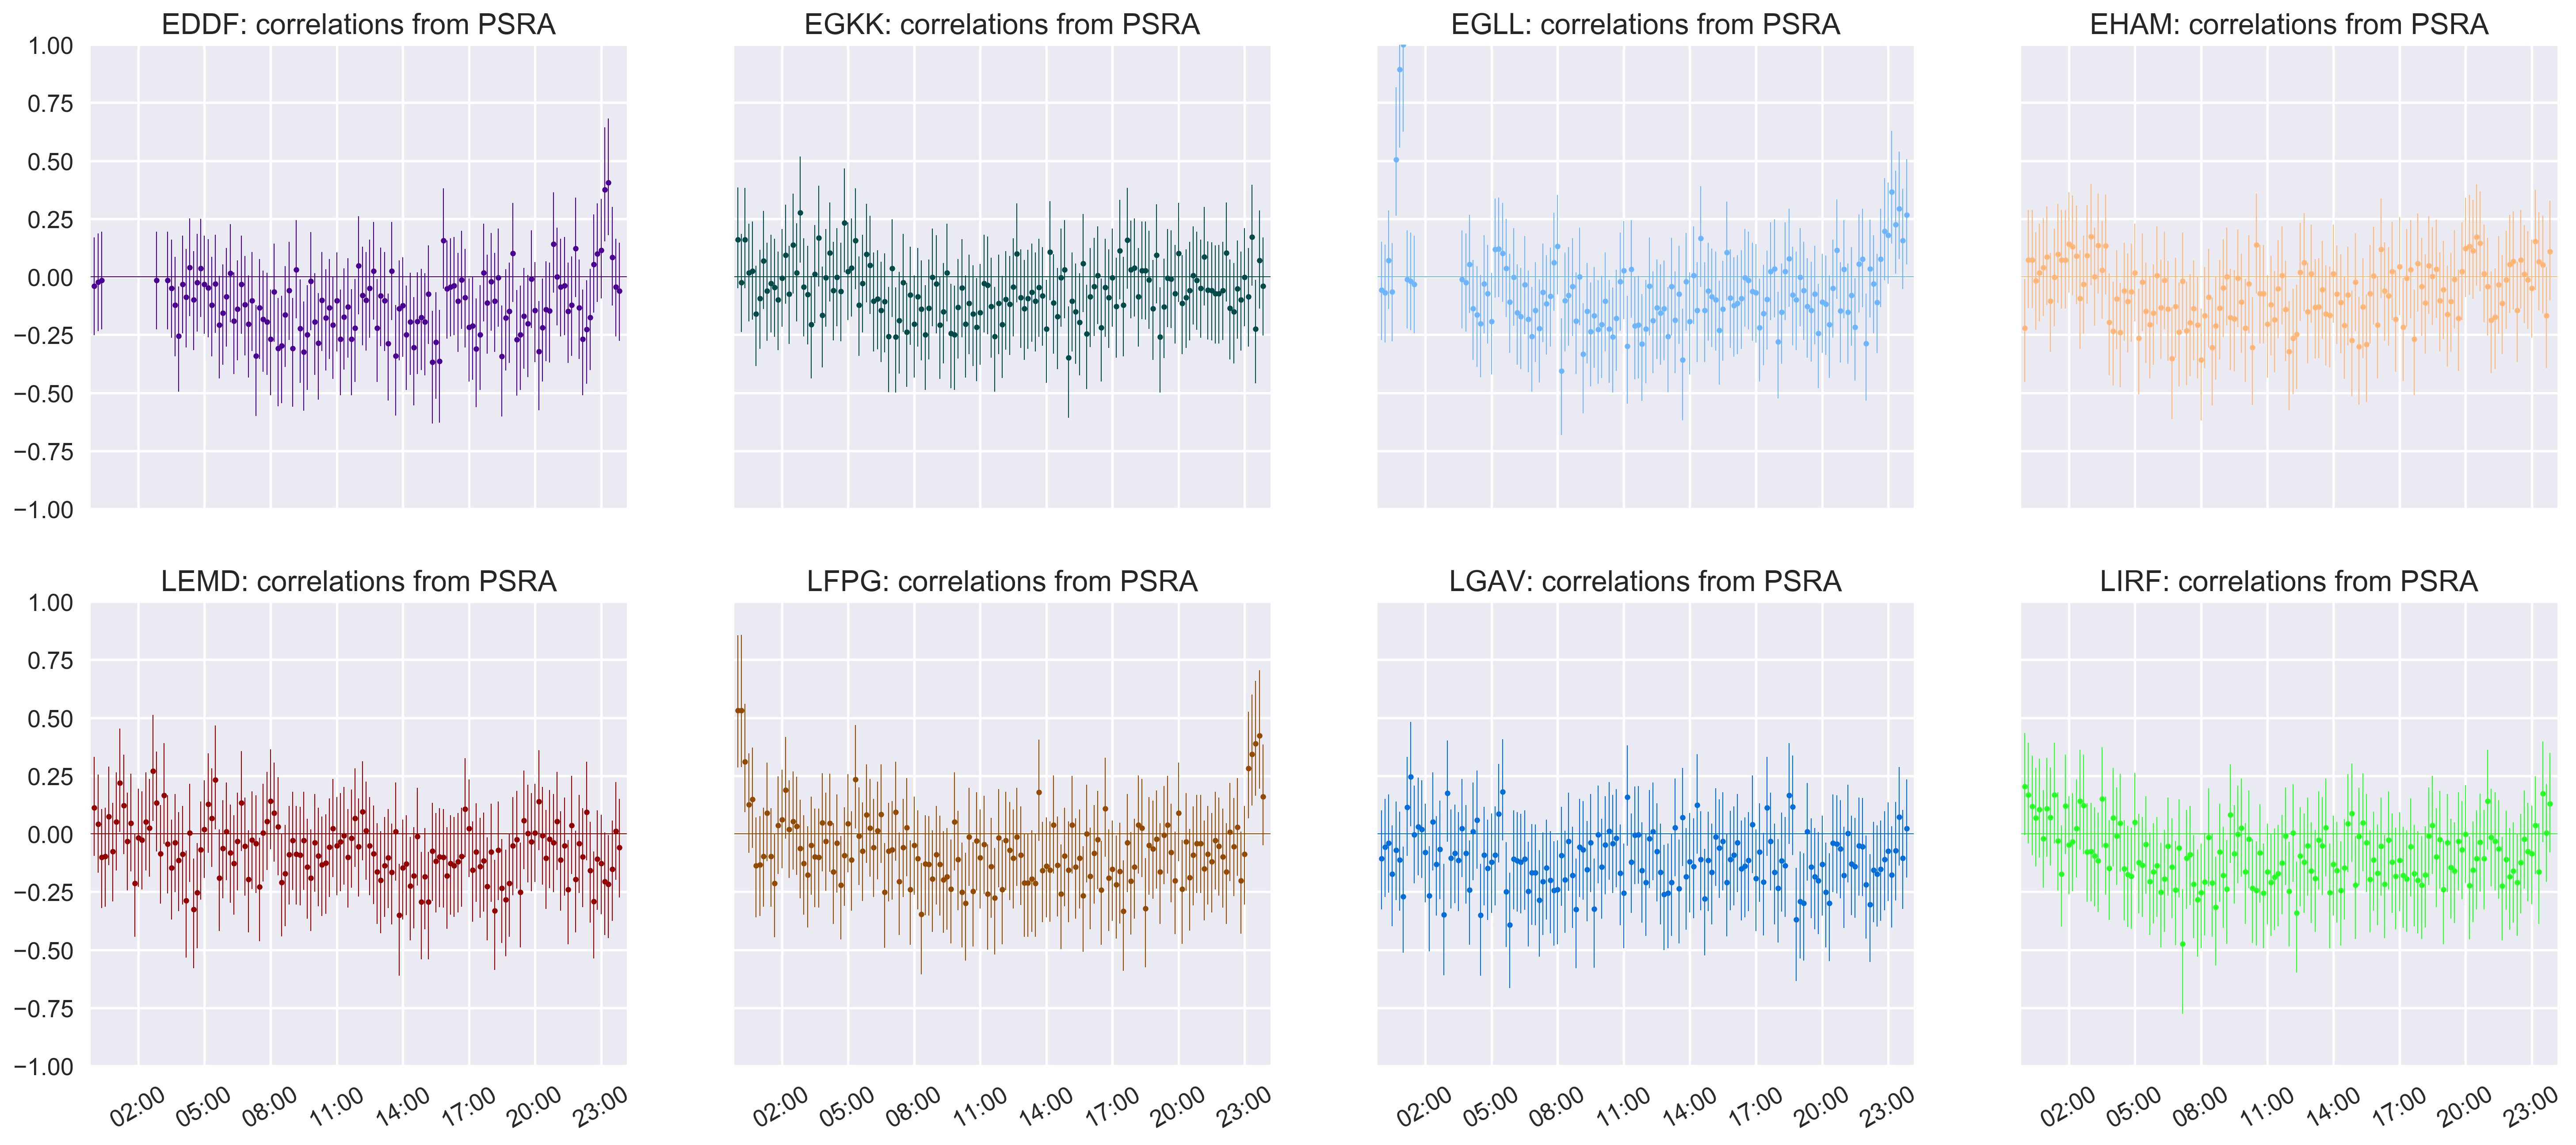
\includegraphics[width=.9\textwidth]{correlations_psra}
\end{frame}

\begin{frame}[t]\frametitle{Conclusions}
    \begin{itemize}
        \item PSRA describes better the inbound flow than Poisson arrivals
        \item Poisson arrivals lead to \alert{overestimation of the queue}
        \item Only advantage of Poisson is mathematical tractability
        \item If time scale is small, \alert{only the transient matters, \emph{i.e. no benefit}}
        \item PSRA are difficult to tackle, but efficient approximation schemes are possible, see Lancia et al (2017) \url{https://arxiv.org/abs/1302.1999}
    \end{itemize}

    \begin{alertblock}{Acknowlegments}
        Lorenzo Capanna and Luigi De Giovanni for their help with querying the DDR database
    \end{alertblock}

    \begin{alertblock}{Preprint}
        Lancia, Lulli (2017) Data-driven modelling and validation of aircraft inbound-stream at some major European airports \url{https://arxiv.org/abs/1708.02486}
    \end{alertblock}
\end{frame}


\end{document}
